\section{Ethinorbital}
\authors{Atousa Seyedian, Gala Gottschalg}
 
\begin{dsafigure}
 \centering
 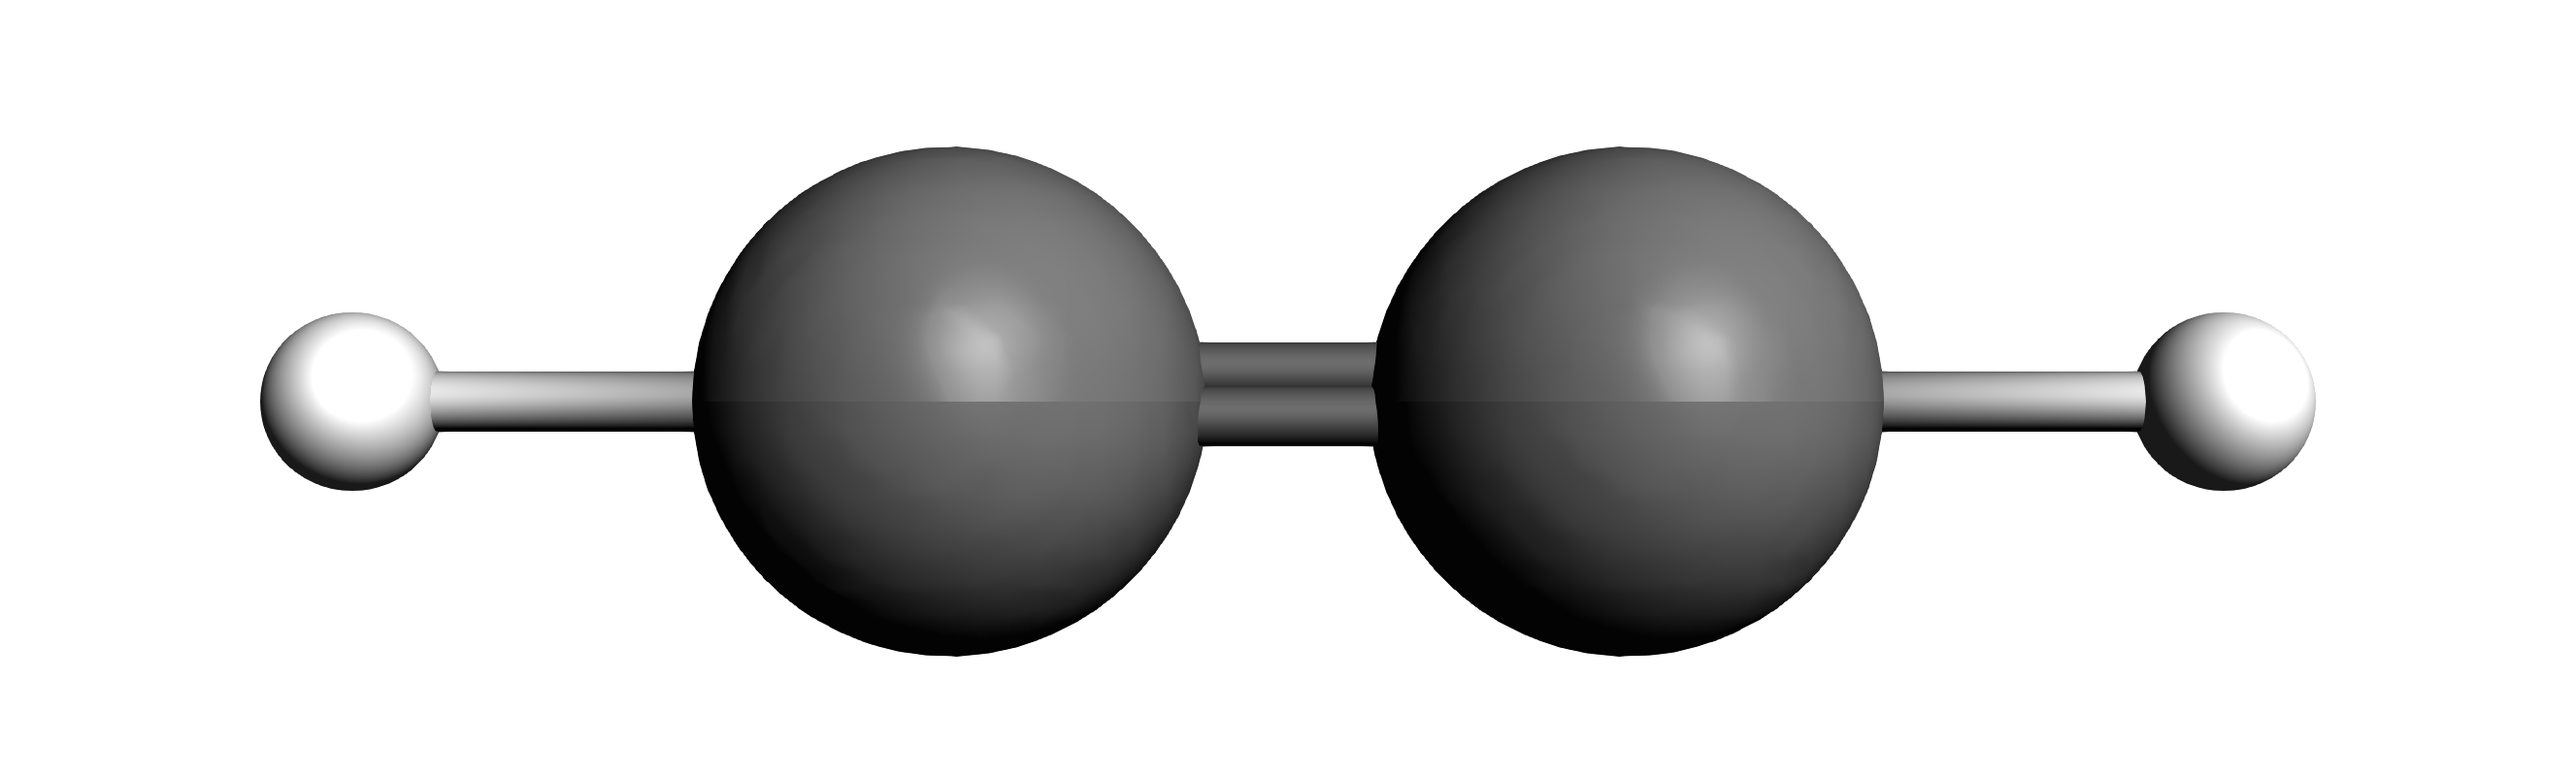
\includegraphics[width=\columnwidth]{ethin.png} 
 \caption{Molekülstruktur des Ethinmoleküls mit Dreifachbindung \cite{ADF2017authors}.}
 \label{dsafigure}
\end{dsafigure} 

Das Ethin-Molekül besitzt eine lineare Struktur. Die beiden 2$p_y$- und 2$p_z$-Orbitale stehen orthogonal zueinander und bilden zwei $\pi$-Bindungen.

\begin{dsafigure}
 \centering
 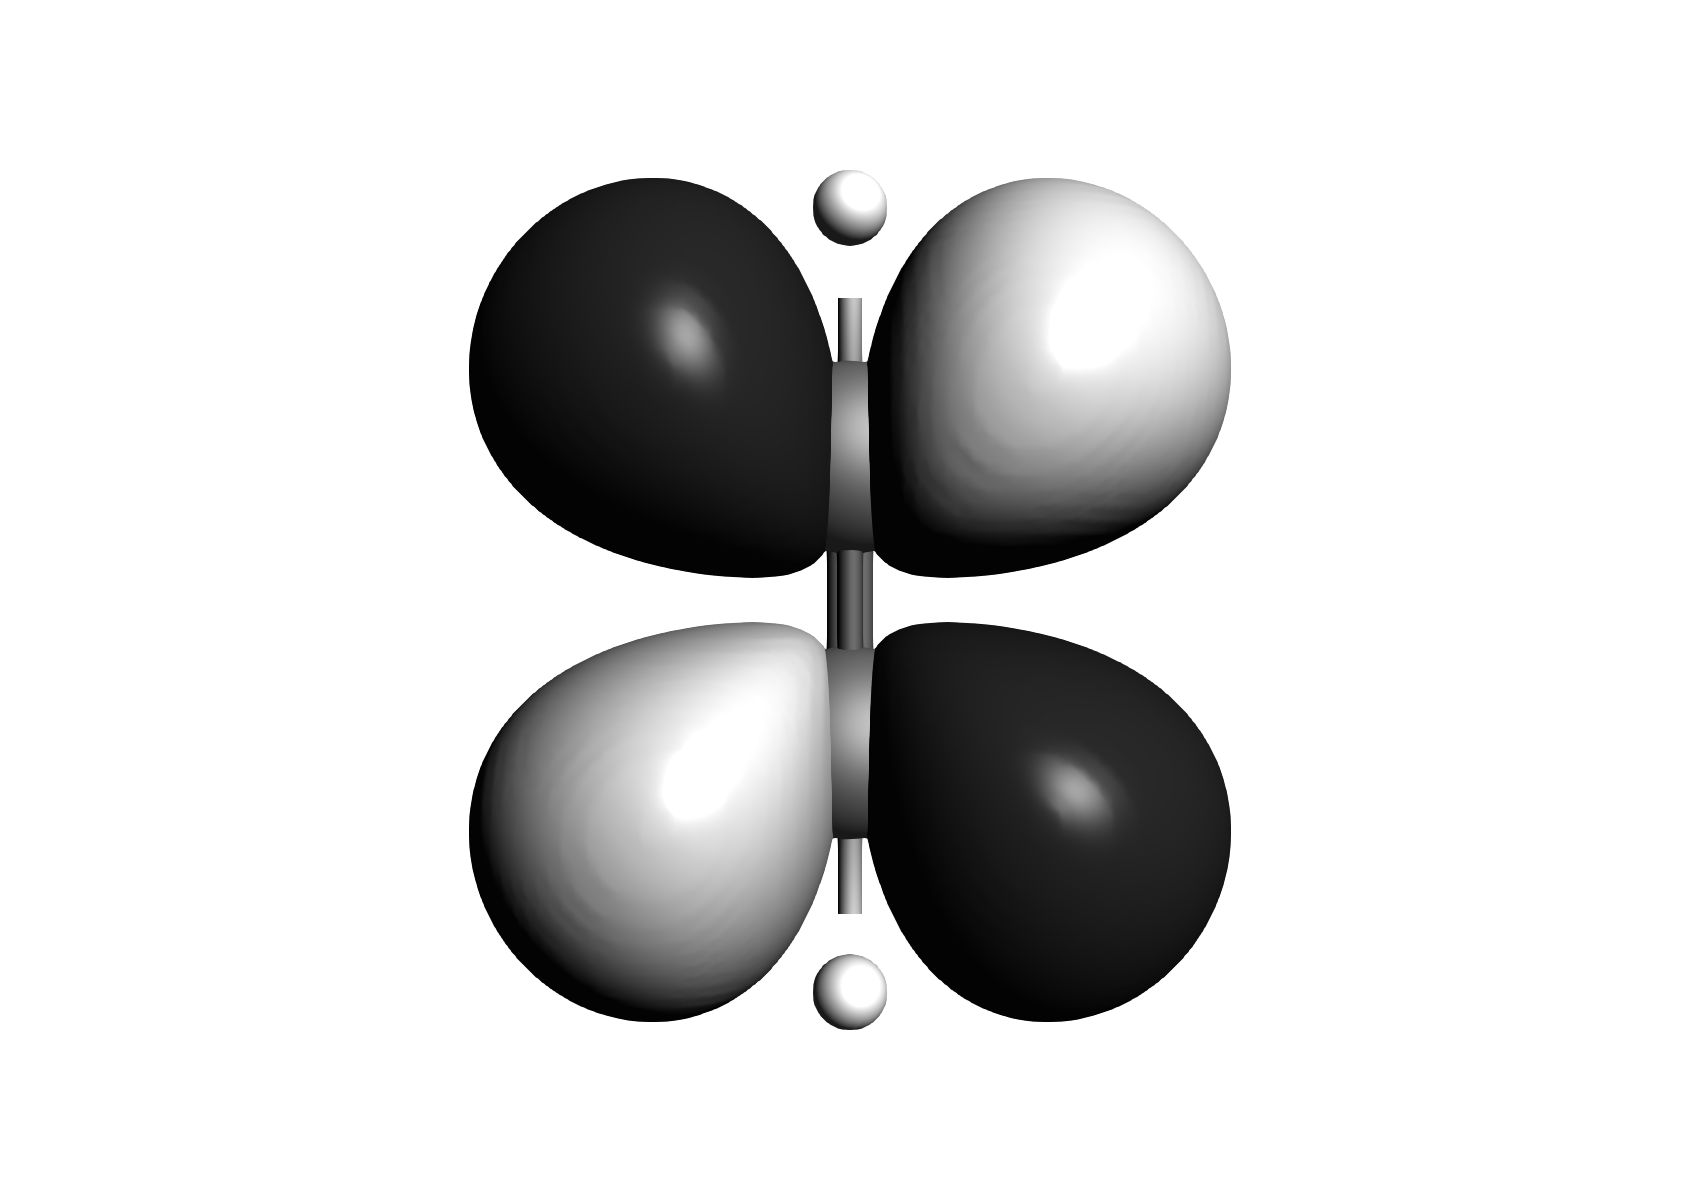
\includegraphics[width=\columnwidth]{ethin2.png}
 \caption{Ein LUMO des Ethins entlang der Bindungsachse \cite{ADF2017authors}.}
 \label{dsafigure:Ethinorbital1}
\end{dsafigure}
 
Wenn man nun die Abbildungen von HOMO und LUMO vergleicht, kann man erkennen, dass beim LUMO in Abbildung \ref{dsafigure:Ethinorbital1} eine Knotenebene orthogonal zur Bindungsachse zwischen den Kohlenstoffatomen vorhanden ist, wodurch sich das Vorzeichen ändert. Entsprechend folgt, dass das LUMO antibindend ist.

Im Modell der Molekülorbitale lässt sich die relative Bindungsstärke durch eine geringe Interferenz der $p$-Orbitale in der $\pi$-Bindung deuten.

\begin{dsafigure}
 \centering
 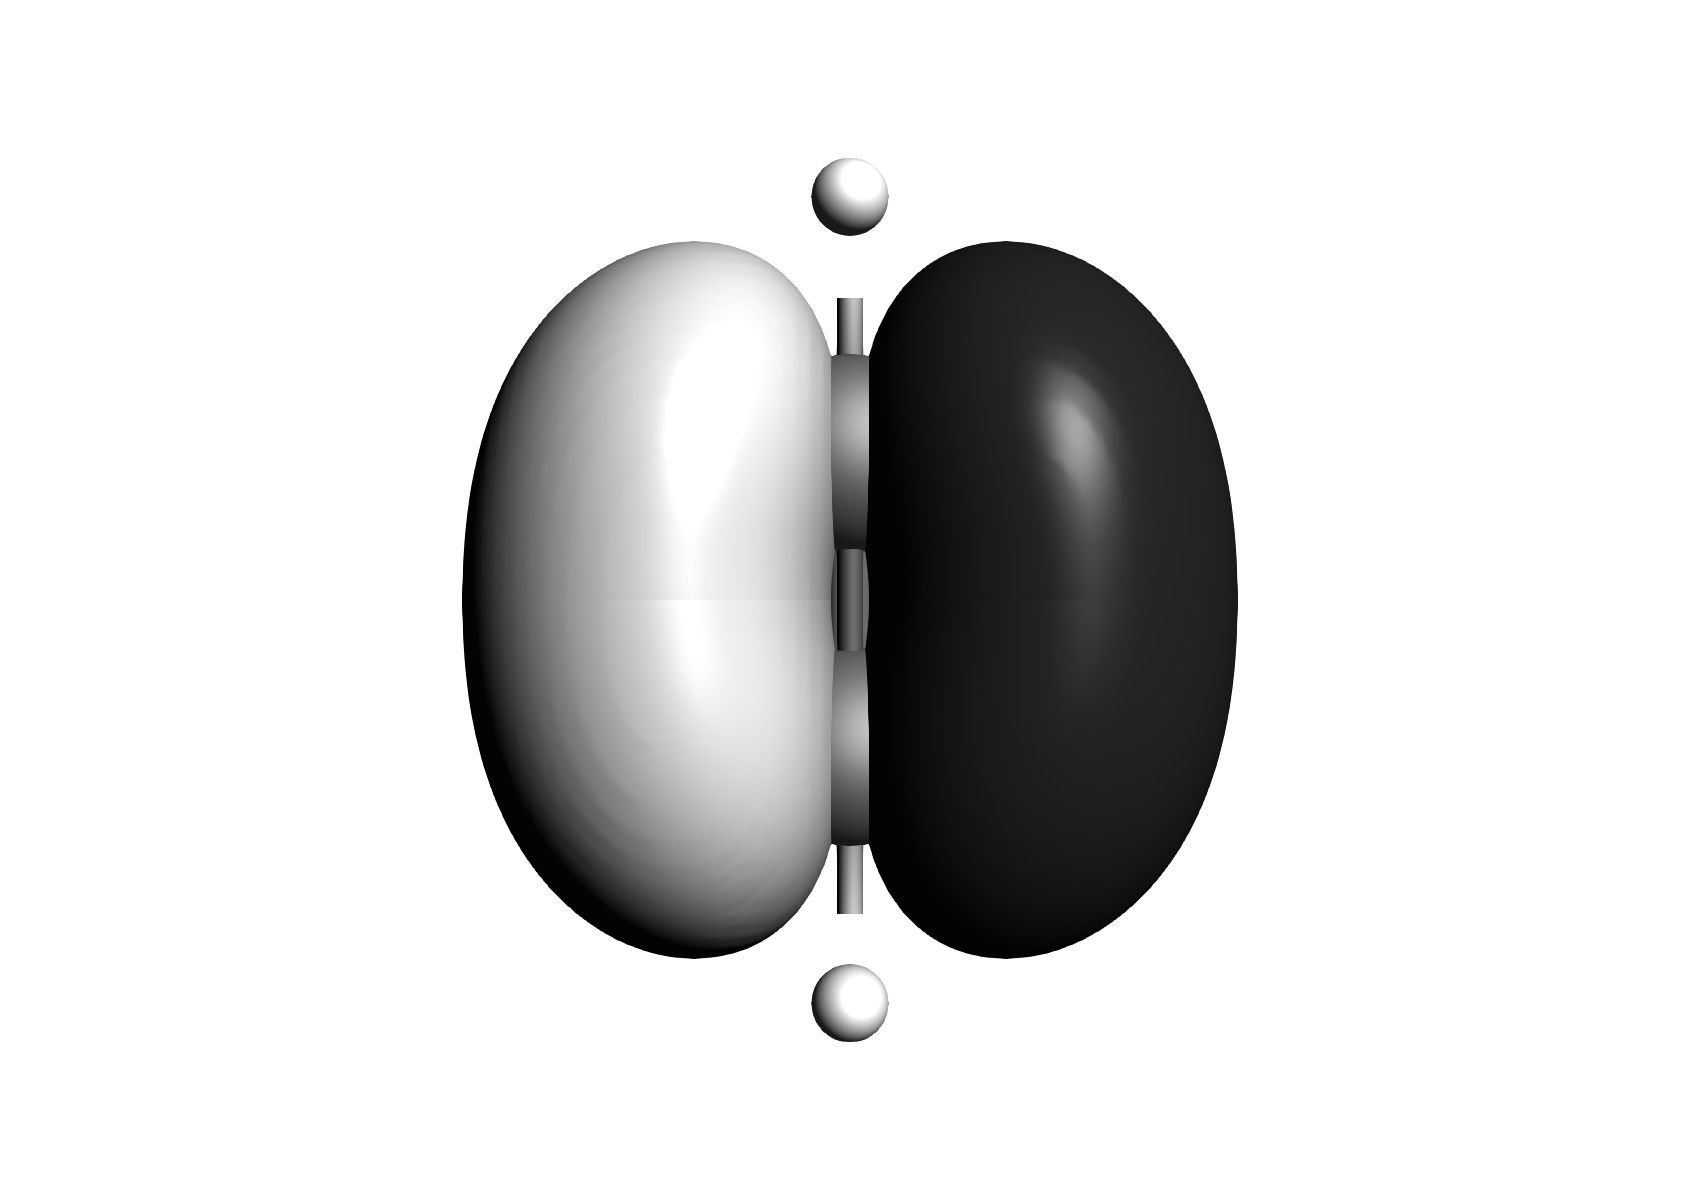
\includegraphics[width=\columnwidth]{help.png}
 \caption{Ein HOMOdes Ethins entlang derBindungsachse \cite{ADF2017authors}.}
 \label{dsafigure:Ethinorbital2}
\end{dsafigure}

Im Gegensatz dazu lässt sich beim HOMO in Abbildung \ref{dsafigure:Ethinorbital2} keine Knotenebene ausmachen, da sich das Vorzeichen nicht ändert und das HOMO bindend ist.
Alle Abbildungen wurden mit dem quantenmechanischen Programm ADF erstellt. Die Molekülorbitale sind mit DFT (DZ/B3LYP) berechnet worden, nachdem die Molekülgeometrie mit einem Kraftfeld optimiert wurde.
